\documentclass[10pt,letterpaper]{article}
\usepackage[margin=0.9in]{geometry}
\usepackage[T1]{fontenc}
\usepackage{lmodern,microtype}
\usepackage{graphicx,booktabs,amsmath,float}
\usepackage{tikz}
\usetikzlibrary{positioning}
\usepackage[colorlinks=true,linkcolor=blue!50!black]{hyperref}
\setlength{\parskip}{4pt}
\setlength{\parindent}{0pt}

\title{\textbf{ESE 5700 Project 2, Part 1}\\RTL Optimization and Synthesis of an NVDLA CMAC Partition}
\author{Seoyoon Park}
\date{\today}

\begin{document}
\maketitle

\begin{table}[H]
\centering
\begin{tabular}{ll}
\toprule
Team member & Contribution \\
\midrule
Seoyoon Park & TODO \\
\bottomrule
\end{tabular}
\end{table}

% ===================== Section 1.1 : Understand the Baseline =====================
% Preamble needs:  \usepackage{graphicx,booktabs,tikz}  \usetikzlibrary{positioning}
% Upload the GTKWave screenshot to Overleaf as  waveform_stripe.png

\section{Understanding the Baseline (1.1)}

\subsection{One stripe in simulation (1.1a)}

Figure~\ref{fig:stripe} shows one stripe from \texttt{make sim} (seed 1, $T = 5.2$\,ns).

\begin{figure}[H]
  \centering
  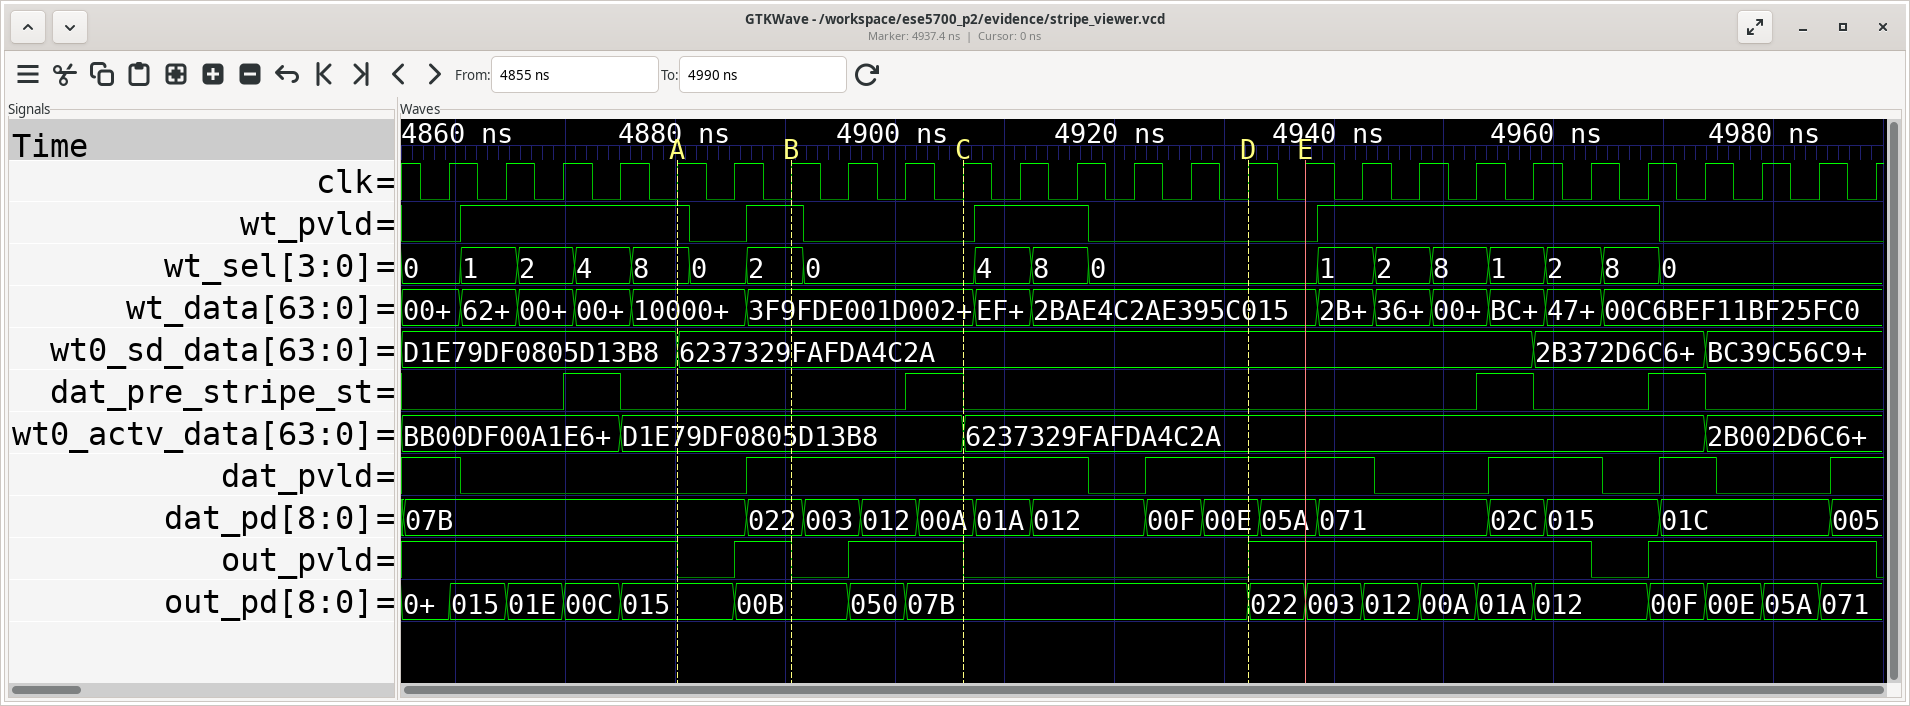
\includegraphics[width=\linewidth]{waveform_stripe.png}
  \caption{One stripe, 4855--4990\,ns. A: cell-0 shadow load; B: stripe-start beat sampled;
  C: shadow $\rightarrow$ active copy; D: matching output appears; E: output sampled by the testbench.}
  \label{fig:stripe}
\end{figure}

\begin{itemize}
  \item \textbf{Shadow load (A, 4880.2\,ns).} A weight beat with \texttt{wt\_sel = 1} (cell 0)
        writes \texttt{wt0\_sd\_data = 0x6237329FAFDA4C2A}. The active weights do not change.
  \item \textbf{Stripe start (B, 4890.6\,ns).} The data beat with \texttt{dat\_pd = 0x022}
        (bit 5 = stripe start) is sampled.
  \item \textbf{Swap (C, 4906.2\,ns).} \texttt{dat\_pre\_stripe\_st} is high and
        \texttt{wt0\_actv\_data} takes the value loaded at A. Meanwhile, weights for the
        next stripe (\texttt{wt\_sel = 4, 8, 1, 2, \ldots}) keep arriving into the shadow registers.
  \item \textbf{Latency (B $\rightarrow$ E).} \texttt{out\_pd = 0x022} appears at D and is
        sampled at E (4937.4\,ns):
        $L = (4937.4 - 4890.6)/5.2 = 9$ cycles, matching the testbench report.
\end{itemize}

\subsection{Pipeline and flip-flop count (1.1b)}

Figure~\ref{fig:pipe} names every register stage. Inside NVDLA the tag (\texttt{pd}, \texttt{pvld})
takes only 6 cycles, so \texttt{cmac\_top} adds 3 registers to realign it with the data.

\begin{figure}[H]
\centering
\resizebox{\linewidth}{!}{%
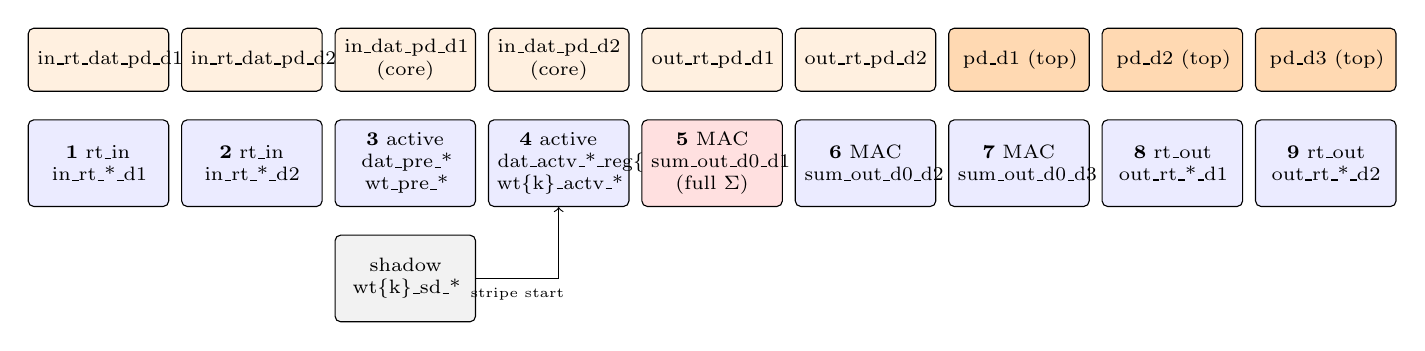
\begin{tikzpicture}[
  st/.style={draw, rounded corners=2pt, minimum height=1.1cm, text width=1.55cm,
             align=center, font=\scriptsize},
  dat/.style={st, fill=blue!8},
  tag/.style={st, fill=orange!12, minimum height=0.8cm},
  node distance=0.15cm]
  % data path
  \node[dat] (d1) {\textbf{1} rt\_in\\in\_rt\_*\_d1};
  \node[dat, right=of d1] (d2) {\textbf{2} rt\_in\\in\_rt\_*\_d2};
  \node[dat, right=of d2] (d3) {\textbf{3} active\\dat\_pre\_*\\wt\_pre\_*};
  \node[dat, right=of d3] (d4) {\textbf{4} active\\dat\_actv\_*\_reg\{k\}\\wt\{k\}\_actv\_*};
  \node[dat, right=of d4, fill=red!12] (d5) {\textbf{5} MAC\\sum\_out\_d0\_d1\\(full $\Sigma$)};
  \node[dat, right=of d5] (d6) {\textbf{6} MAC\\sum\_out\_d0\_d2};
  \node[dat, right=of d6] (d7) {\textbf{7} MAC\\sum\_out\_d0\_d3};
  \node[dat, right=of d7] (d8) {\textbf{8} rt\_out\\out\_rt\_*\_d1};
  \node[dat, right=of d8] (d9) {\textbf{9} rt\_out\\out\_rt\_*\_d2};
  % shadow weights (off the data path)
  \node[st, below=0.35cm of d3, fill=gray!10] (sd) {shadow\\wt\{k\}\_sd\_*};
  \draw[->] (sd.east) -| node[pos=0.25, below, font=\tiny]{stripe start} (d4.south);
  % tag path
  \node[tag, above=0.35cm of d1] (t1) {in\_rt\_dat\_pd\_d1};
  \node[tag, above=0.35cm of d2] (t2) {in\_rt\_dat\_pd\_d2};
  \node[tag, above=0.35cm of d3] (t3) {in\_dat\_pd\_d1\\(core)};
  \node[tag, above=0.35cm of d4] (t4) {in\_dat\_pd\_d2\\(core)};
  \node[tag, above=0.35cm of d5] (t5) {out\_rt\_pd\_d1};
  \node[tag, above=0.35cm of d6] (t6) {out\_rt\_pd\_d2};
  \node[tag, above=0.35cm of d7, fill=orange!30] (t7) {pd\_d1 (top)};
  \node[tag, above=0.35cm of d8, fill=orange!30] (t8) {pd\_d2 (top)};
  \node[tag, above=0.35cm of d9, fill=orange!30] (t9) {pd\_d3 (top)};
\end{tikzpicture}}
\caption{Baseline pipeline, one column per clock cycle. Blue: data/weights. Orange: tag and valid.
The whole multiply-add sits between stages 4 and 5.}
\label{fig:pipe}
\end{figure}

\begin{table}[H]
\centering
\small
\begin{tabular}{llrr}
\toprule
Module & Registers (bits) & Hand count & Genus \\
\midrule
rt\_in     & $2 \times [\,(1+8+9+64)_{dat} + (1+8+4+64)_{wt}\,]$ & 318  & 318 \\
active     & $76 + 4(73) + 4(81) + 75 + 4(80) + 1$             & 1088 & 809 \\
MAC (one)  & $3 \times (19 + 1)$                               & 60   & 60  \\
MAC (four) & $4 \times 60$                                     & 240  & 240 \\
rt\_out    & $2(1+4+9+76) + 3_{done} + 2_{cfg}$                & 185  & 183 \\
core local & $2 \times (9+1)$                                  & 20   & 20  \\
cfg        & 5 one-bit registers                               & 5    & 0   \\
cmac\_top  & $3 + 3 \times 9$                                  & 30   & 30  \\
\midrule
Total      &                                                   & 1886 & 1600 \\
\bottomrule
\end{tabular}
\caption{Flip-flops by submodule. Genus counts are from the baseline synthesis in Section 1.2.}
\label{tab:ff}
\end{table}

The 286-FF difference has three causes:
\begin{itemize}
  \item \textbf{Merged duplicates ($-279$).} \texttt{active} keeps four identical copies of the
        activation registers (one per MAC cell, to limit fanout). Genus merges them and the
        eight identical per-lane valid bits: $4(80) \rightarrow 73$ saves 247. Each active-weight
        bank's 9 identical valid bits become 1, saving $4 \times 8 = 32$.
  \item \textbf{Constant registers ($-7$).} \texttt{cmac\_top} ties the configuration inputs off,
        so the 5 \texttt{cfg} registers and 2 \texttt{cfg\_*\_d1} registers in \texttt{rt\_out}
        are constant and removed.
  \item \textbf{Not counted.} Declared-but-unassigned \texttt{reg}s and the simulation-only
        \texttt{dbg\_out\_*} registers produce no flip-flops.
\end{itemize}

\subsection{The three \texttt{sum\_out\_d0\_d*} stages (1.1c)}

\texttt{sum\_out\_d0\_d1} stores the \emph{completed} 19-bit dot product;
\texttt{sum\_out\_d0\_d2} and \texttt{sum\_out\_d0\_d3} only delay that same value by one cycle each
(with \texttt{pp\_pvld\_d0\_d*} as valids). All eight multiplies and the full adder tree therefore
sit between the active registers (stage 4) and \texttt{sum\_out\_d0\_d1} (stage 5), which is the
critical path. The extra two stages add latency but cut no logic.
The RTL comment ``add pipeline for retiming'' shows they were meant to be pushed back into the
arithmetic by register retiming. Genus does not do this unless retiming is enabled, and the load
enables on these registers make retiming harder.


\end{document}
